% !TEX root = ../relatorio.tex

\subsection{Arquitetura de DSP}

A fim cumprir os objetivos listados acima, proponho a arquitetura descrita na figura \ref{fig:arquitetura}.

A aplicação processará sequencialmente as amostras de entrada e aplicará um filtro simplificado calculado a partir de 10 filtros passa-faixa dividindo o espectro entre as frequências requeridas no projeto. Para o cálculo dos valores do gráfico de barras, aplicaremos periodicamente uma FFT, somando as energias das faixas especificadas.

\begin{figure}[h]
    \centering
    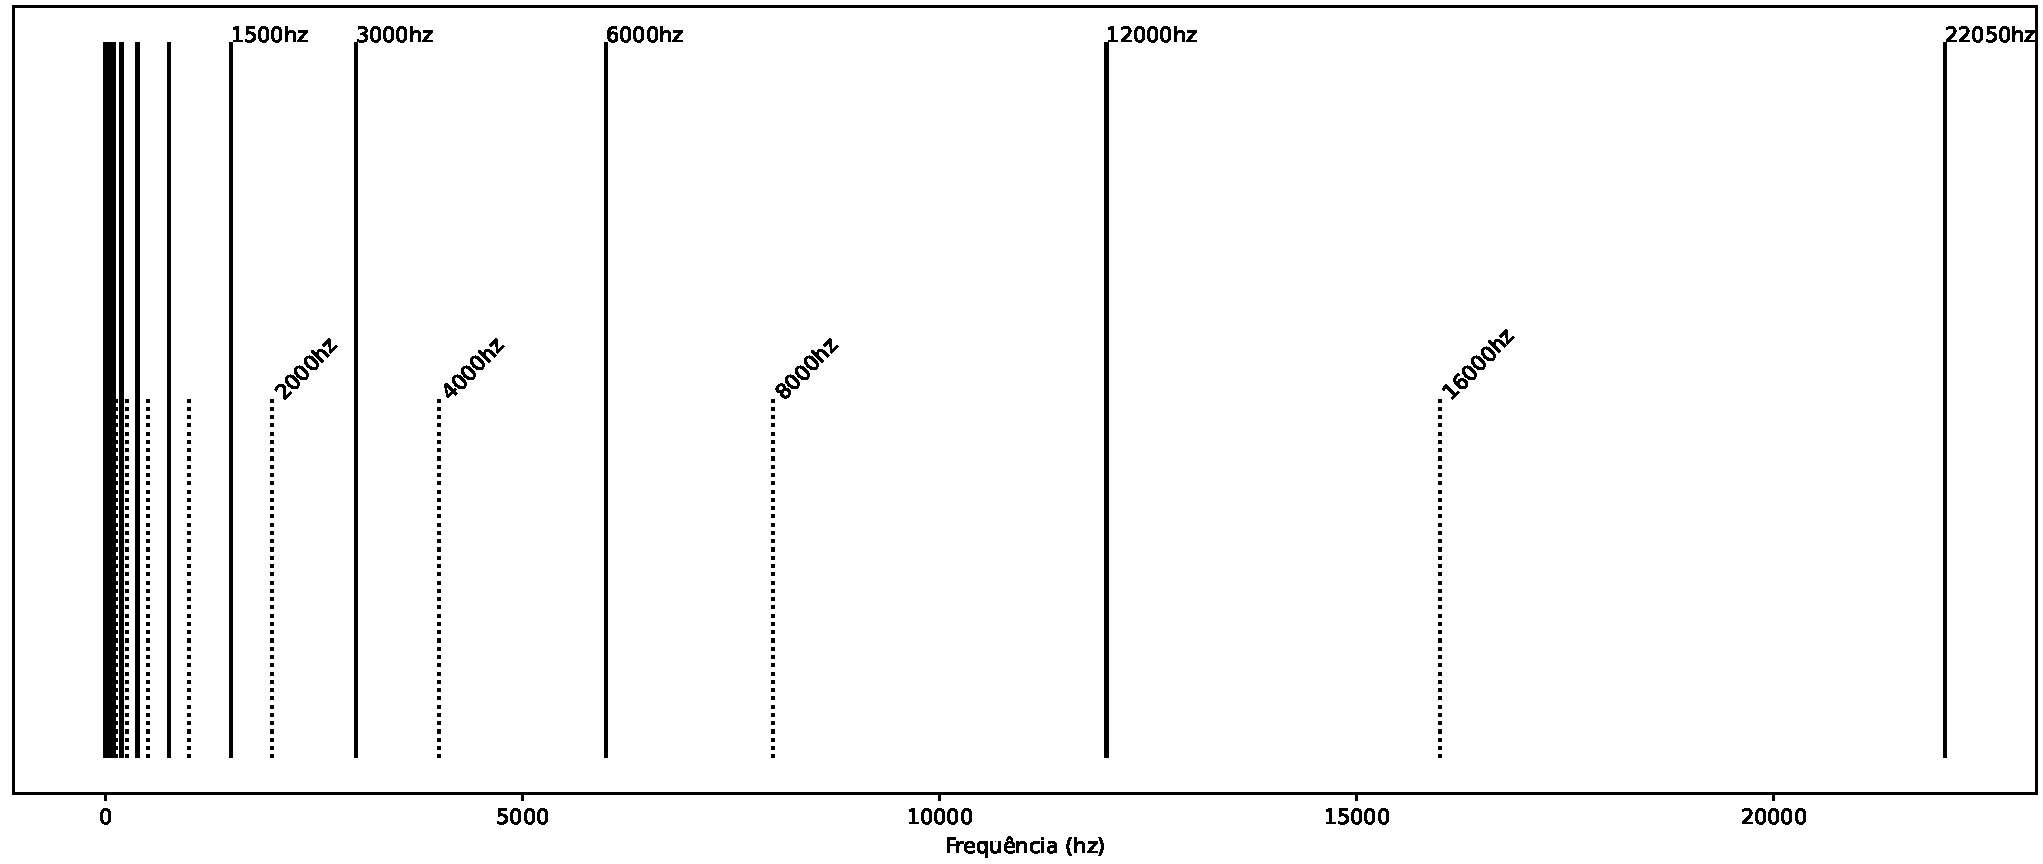
\includegraphics[scale=.45]{fig/Bands.pdf}\\
    \small{Pontilhadas: frequências "centrais" das bandas}\\
    \small{Sólidas: frequências-limite das bandas}
    \caption{Bandas de filtragem}
    \label{fig:bandas}
\end{figure}

\begin{figure}[h]
    \centering
    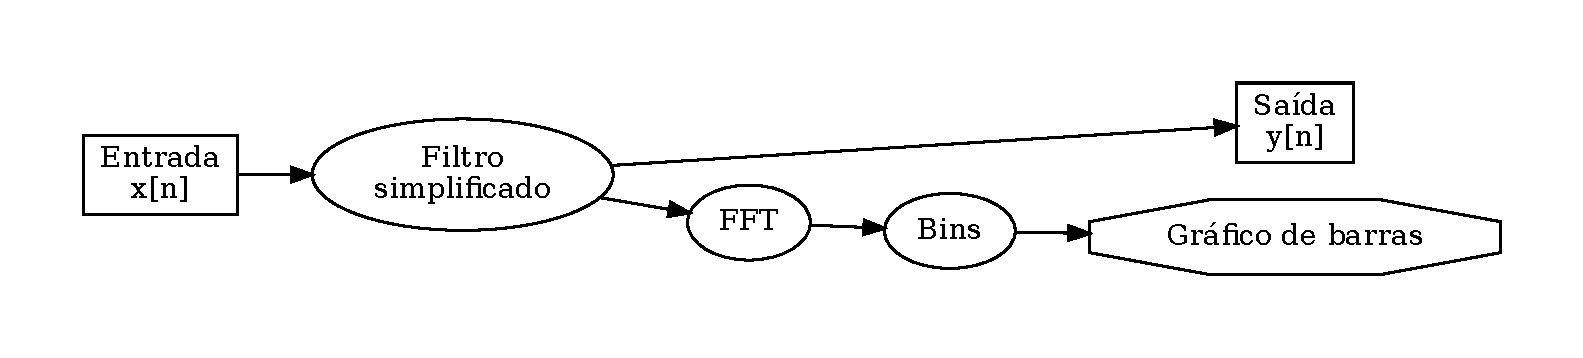
\includegraphics[scale=0.5]{fig/arquiteturafft.pdf}
    \caption{Aquitetura proposta}
    \label{fig:arquitetura}
\end{figure}
\break
\subsection{Arquitetura da aplicação}


A aplicação se dividirá em três componentes principais:
\begin{multicols}{2}   
    \begin{itemize}
        \item Provedor de informação dos sliders;
        \begin{itemize}
            \item Codificado em Python;
            \item Apresentará a interface de alteração dos filtros para o usuário;
            \item Proverá os coeficientes do filtro para o processador de sinais via FIFO/Pipe UNIX.
        \end{itemize}
        \item Host de filtragem;
        \begin{itemize}
            \item Codificado em C;
            \item Receberá coeficientes de filtragem via FIFO/Pipe UNIX;
            \item Receberá um feed de som do PulseAudio, aplicará o filtro FIR caracterizado pelos parâmetros guardados e enviará um feed de som de volta ao PulseAudio;
        \end{itemize}
        \columnbreak
        \item Visualizador de gráfico de barras.
        \begin{itemize}
            \item Codificado em Python;
            \item Receberá um feed de som do PulseAudio e gerará um gráfico de barras de intensidade de cada banda.
        \end{itemize}
    \end{itemize}
\end{multicols}
\begin{figure}[H]
    \centering
    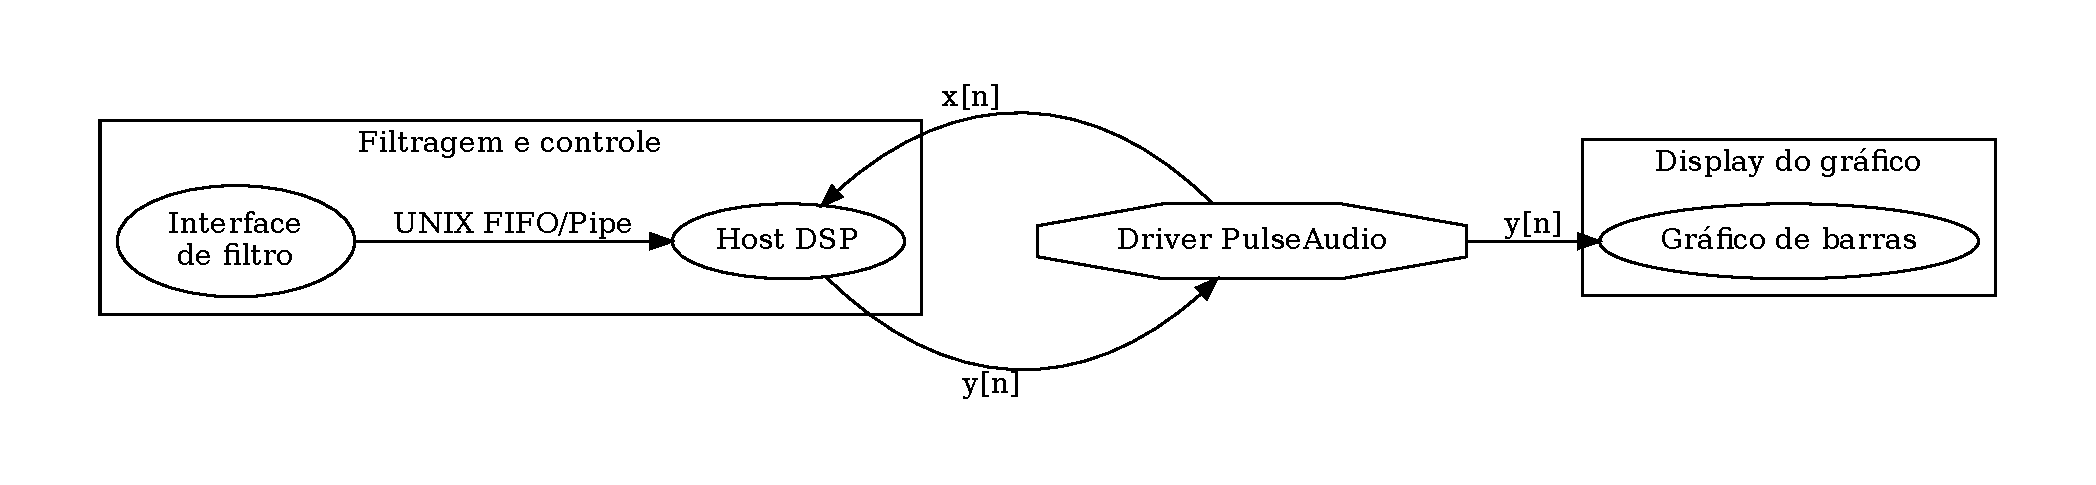
\includegraphics[scale=0.45]{fig/app.pdf}
    \caption{Processos e conexões relevantes}
    \label{fig:app}
\end{figure}


Destes processos, dois grupos são basicamente independentes:

\begin{multicols}{2}
    \begin{itemize}
        \item Processos de controle e filtragem
        \begin{itemize}
            \item Lidam com a filtragem do áudio e configuração do filtro;
            \item Lidam com a interação com o usuário.
        \end{itemize}
        \columnbreak
        \item Processo de display do gráfico
        \begin{itemize}
            \item Lida com o cálculo das intensidades de cada \textit{bin} de frequências.
            \item Lida com a ilustração das intensidades com um gráfico de barras.
        \end{itemize}
    \end{itemize}
\end{multicols}

O isolamento dos dois grupos, bem como o desenho do host de DSP de forma "reativa" (funciona continuamente até que alguma alteração venha da interface, com mínima interrupção) permite que o feed de som seja contínuo, sem falhas provindas de gargalos de processamento, e que o display visual, para o qual continuidade não é tão importante, possa lidar com o feed de som em seu próprio "ritmo".